\documentclass[a4paper]{article}

\usepackage[T1]{fontenc}
\usepackage[italian]{babel}
\usepackage[latin1]{inputenc}
\usepackage{graphicx}
\usepackage{float}
\usepackage[margin=2 cm]{geometry}
\usepackage{multirow}
\usepackage{multicol}
\usepackage{textcomp}
\usepackage{caption}
\author{A. Bordin, G. Cappelli}
\title{Visibile}
\date{4-5 Dicembre 2017}
\newcommand{\minitab}[2][l]{\begin{tabular}#1 #2\end{tabular}}


\begin{document}
	\maketitle
	
	\begin{abstract}
		 
	\end{abstract}
	
	\begin{multicols}{2}
	
\section{Teoria}

\section{Apparato sperimentale}

\section{Presa dati}

\subsection{Taratura attenuatore}

Per prima cosa eseguiamo la taratura dell'attenuatore variabile. in modo tale da avere la curva di conversione fra angolo e potenza. 
Sull'attenuatore � montato un goniometro cos� da permetterci di registrare, attraverso il power meter, la potenza del fascio laser di pompaggio una volta attraversato l'attenuatore. Abbiamo registrato le misure variando l'angolo ogni volta di 2� coprendo i 360� dell'attenuatore.

I valori misurati sono riportati in Tabella \ref{tab:taratura} in Appendice.

Cos� facendo abbiamo ottenuto una curva di conversione (Figura \ref{fig:taratura}) che ci permette, misurando l'angolo a cui `e posizionato il goniometro, di conoscere la potenza incidente sul cristallo. 

Dato che il laser a nostra disposizione � nell'infrarosso, $\lambda$=975.9(2.9) nm, utilizziamo una cartina che rivela l'IR per allineare il laser nel power meter che abbiamo posto ad una distanza di $\sim$1 cm dall'attenuatore.

\end{multicols}

\begin{figure}[H]
\centering
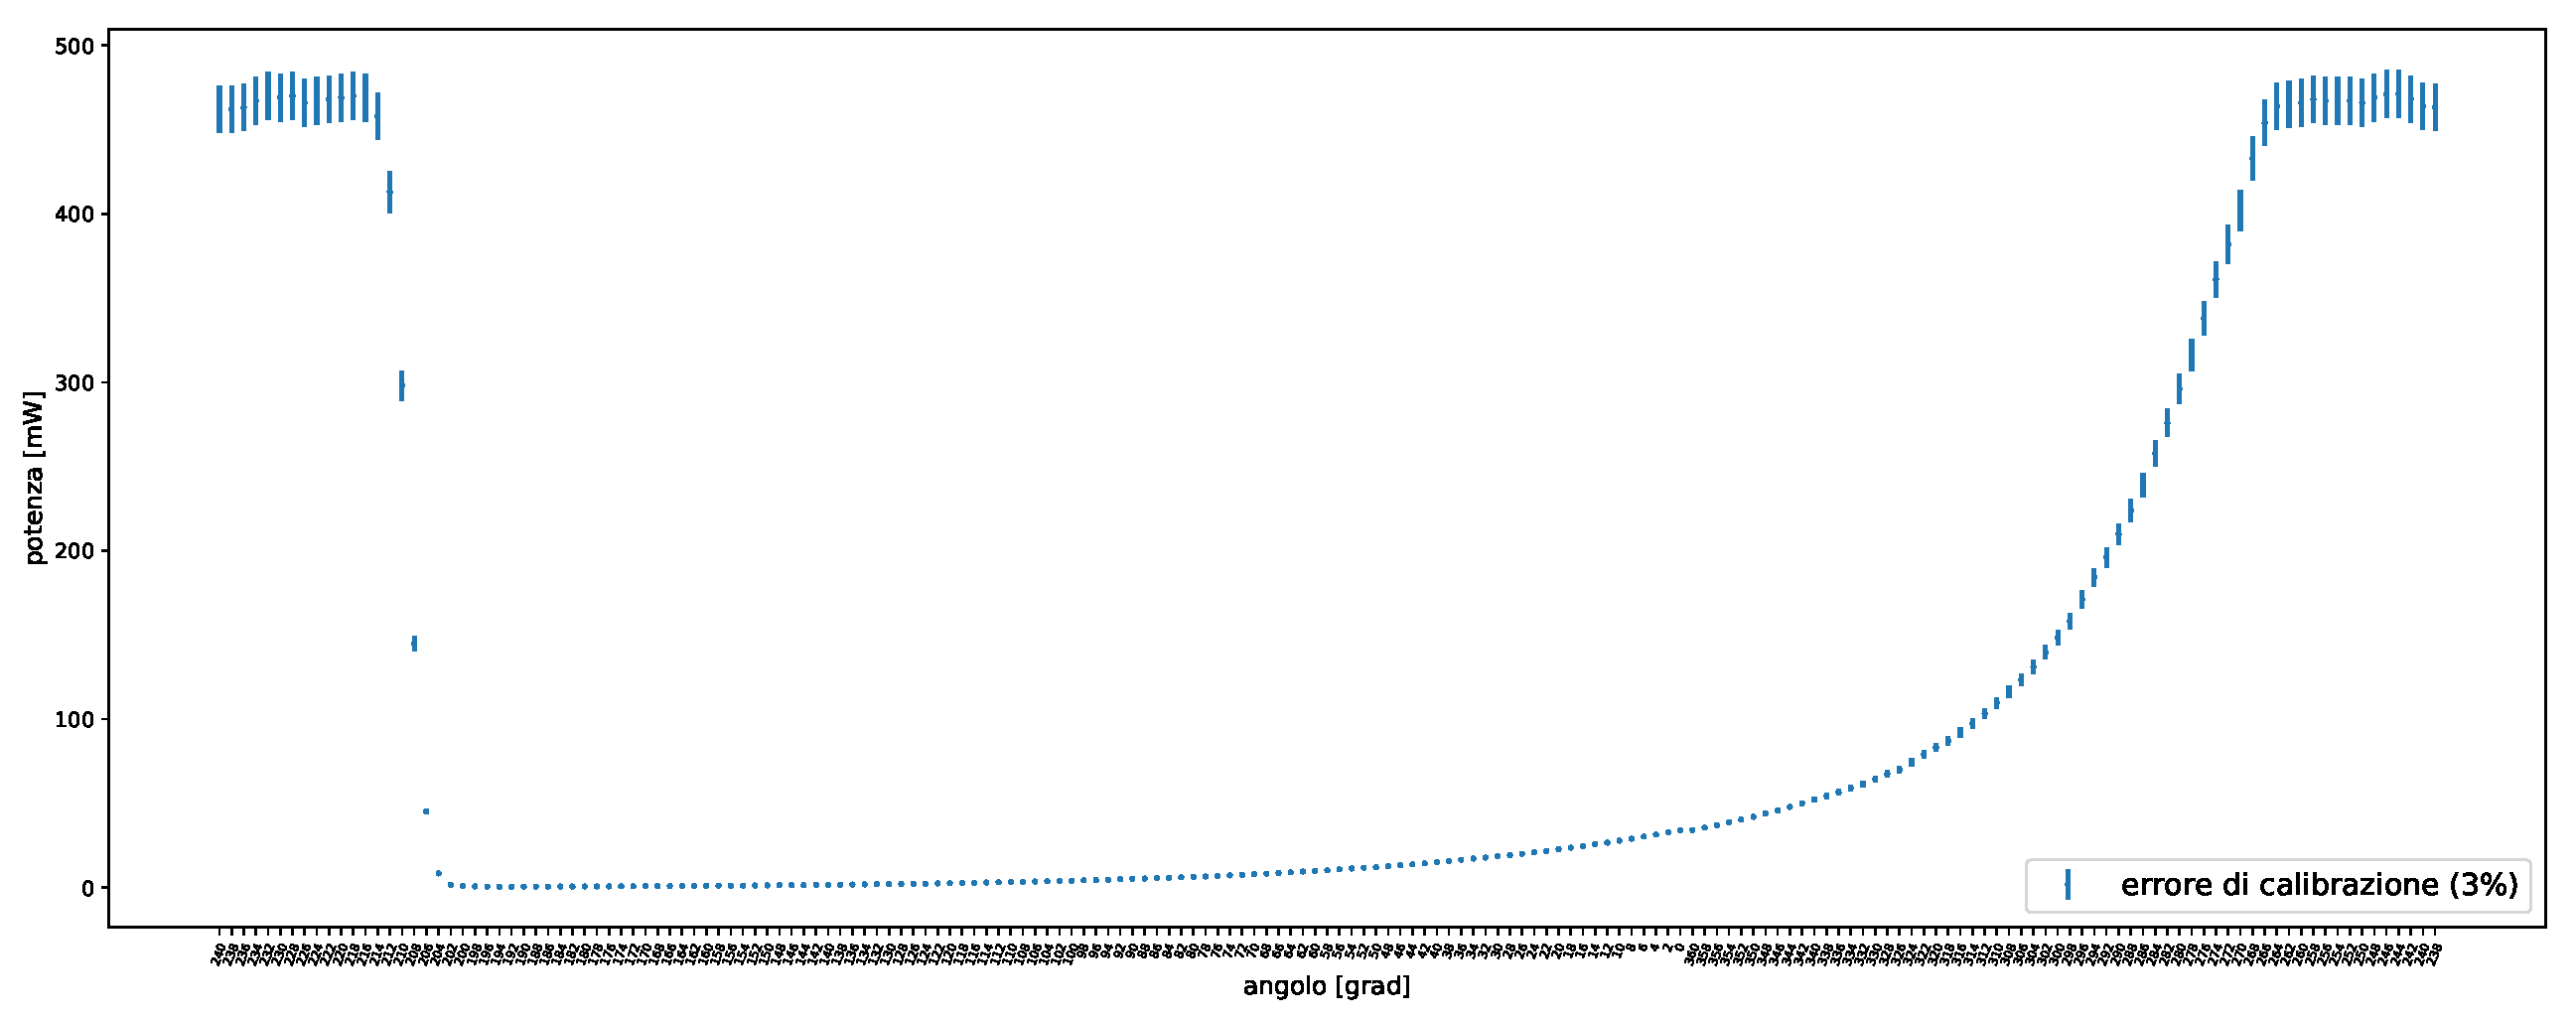
\includegraphics[width=0.9\textwidth]{taratura}
\caption{Taratura dell'attenuatore variabile}
\label{fig:taratura}
\end{figure}

\begin{multicols}{2}

\subsection{Acquisizione segnale}

Una volta effettuata la taratura abbiamo misurato la tensione relativa alla luce emessa dal cristallo in funzione della potenza incidente. 

Per farlo abbiamo utilizzato un oscilloscopio leggendo, attraverso i cursori, l'ampiezza picco picco dell'onda quadra ottenuta utilizzando il chopper impostato ad una frequenza di $\sim$75 Hz.

Prima di registrare le misure ci siamo preoccupati di spegnere la luce ambientale in quanto si vedevano i battimenti con la 50 Hz. Abbiamo quindi utilizzato una pila per illuminare il goniometro presente sull'attenuatore; la luce proveniente dalla pila era irrilevante in quando produceva solamente un offset costante al segnale.

Durante la prima presa dati abbiamo notato che, mentre il massimo restava costante, il minimo del segnale proveniente dal chopper si spostava a causa di effetti 1/f non trascurabili che portavano a variazioni anche del 10\%.
I valori ottenuti sono riportati nella Tabella \ref{tab:primo} in Appendice e in Figura \ref{fig:primo}.

Abbiamo quindi cambiato l'alimentatore del laser per risolvere questo problema e ripetuto le misure senza ottenere per� miglioramenti visibili. I dati relativi a questa seconda presa dati sono riportati nella Tabella \ref{tab:secondo} in Appendice e in Figura \ref{fig:secondo}.

\end{multicols}

\begin{figure}[H]
\centering
\begin{minipage}[c]{\textwidth}
\centering
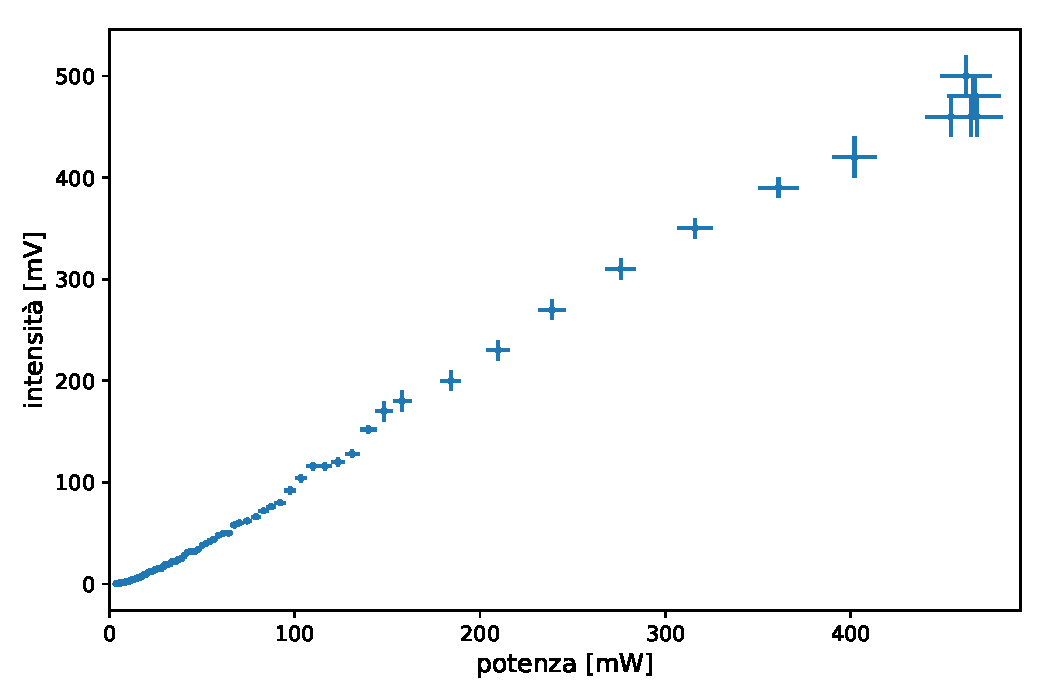
\includegraphics[width=0.9\textwidth]{primo}
\caption{Prima acquisizione. Come errore sulla tensione � riportata la digitalizzazione dell'oscilloscopio, mentre sulla potenza � indicato il 3\% della calibrazione.}
\label{fig:primo}
\end{minipage}
\begin{minipage}[c]{\textwidth}
\centering
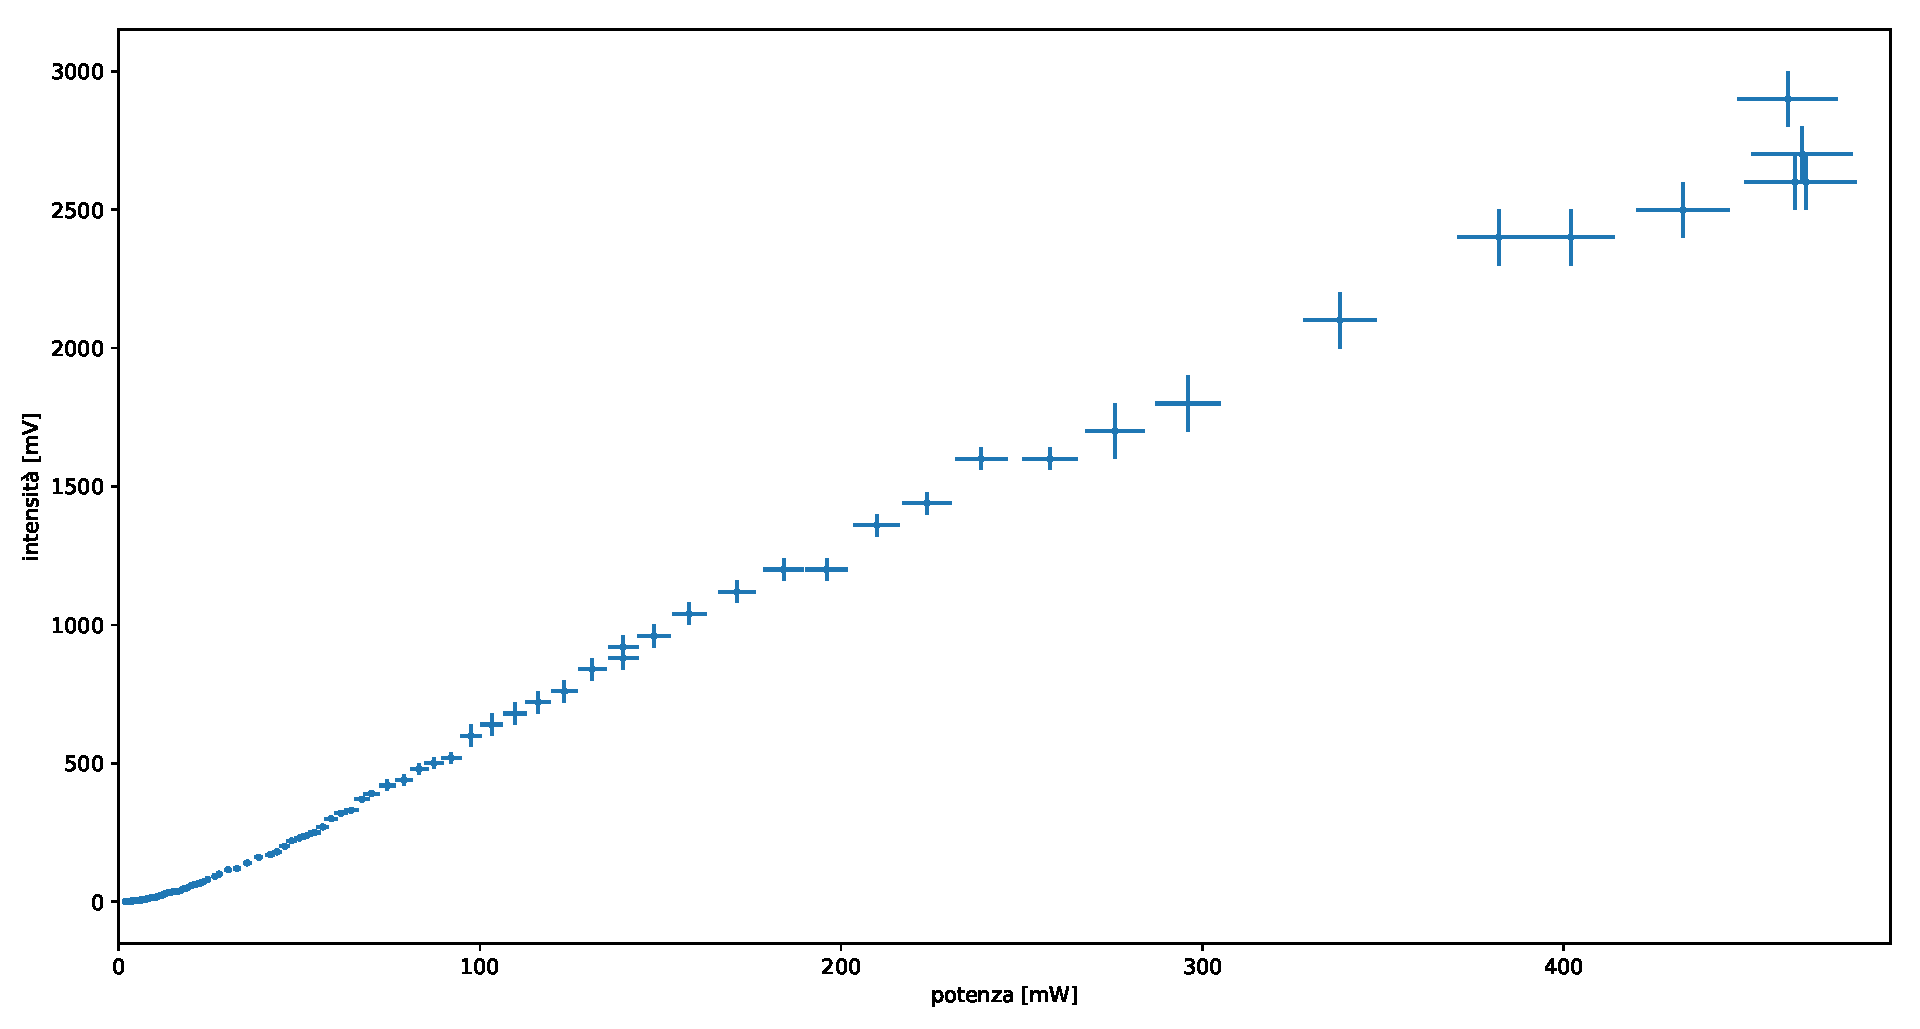
\includegraphics[width=0.9\textwidth]{secondo}
\caption{Seconda acquisizione; eseguita dopo la sostituzione dell'alimentatore del laser di pompa. Per gli errori sono stati usati gli stessi criteri precedenti.}
\label{fig:secondo}
\end{minipage}
\end{figure}

\begin{multicols}{2}

In entrambe le figure si hanno degli andamenti non regolari soprattuto nella zona di medio-alta potenza ed � evidente come la sostituzione dell'alimentatore non abbia portato alcun miglioramento. 

\subsubsection{Discussione degli errori}
In tutte le precedenti figure abbiamo riportato l'errore di calibrazione sulla potenza, che � un errore sistematico. Nelle sezioni successive talvolta � richiesto l'uso di un errore statistico, in tal caso verr� usata la sigma relativa all'errore di digitalizzazione.

\subsection{Acquisizione spettro}

Infine, tramite una fibra ottica, abbiamo portato la luce emessa dal cristallo all'analizzatore di spettro e acquisito lo spettro della radiazione. 

Per evitare la saturazione e quindi l'impossibilit� di visualizzare il picco abbiamo attenuato il laser di pompa. Le misure sono state effettuate con un'integrazione sullo spettrometro di 500 ms e sono riportate in Figura \ref{fig:spettro}.

\end{multicols}

\begin{figure}[H]
\centering
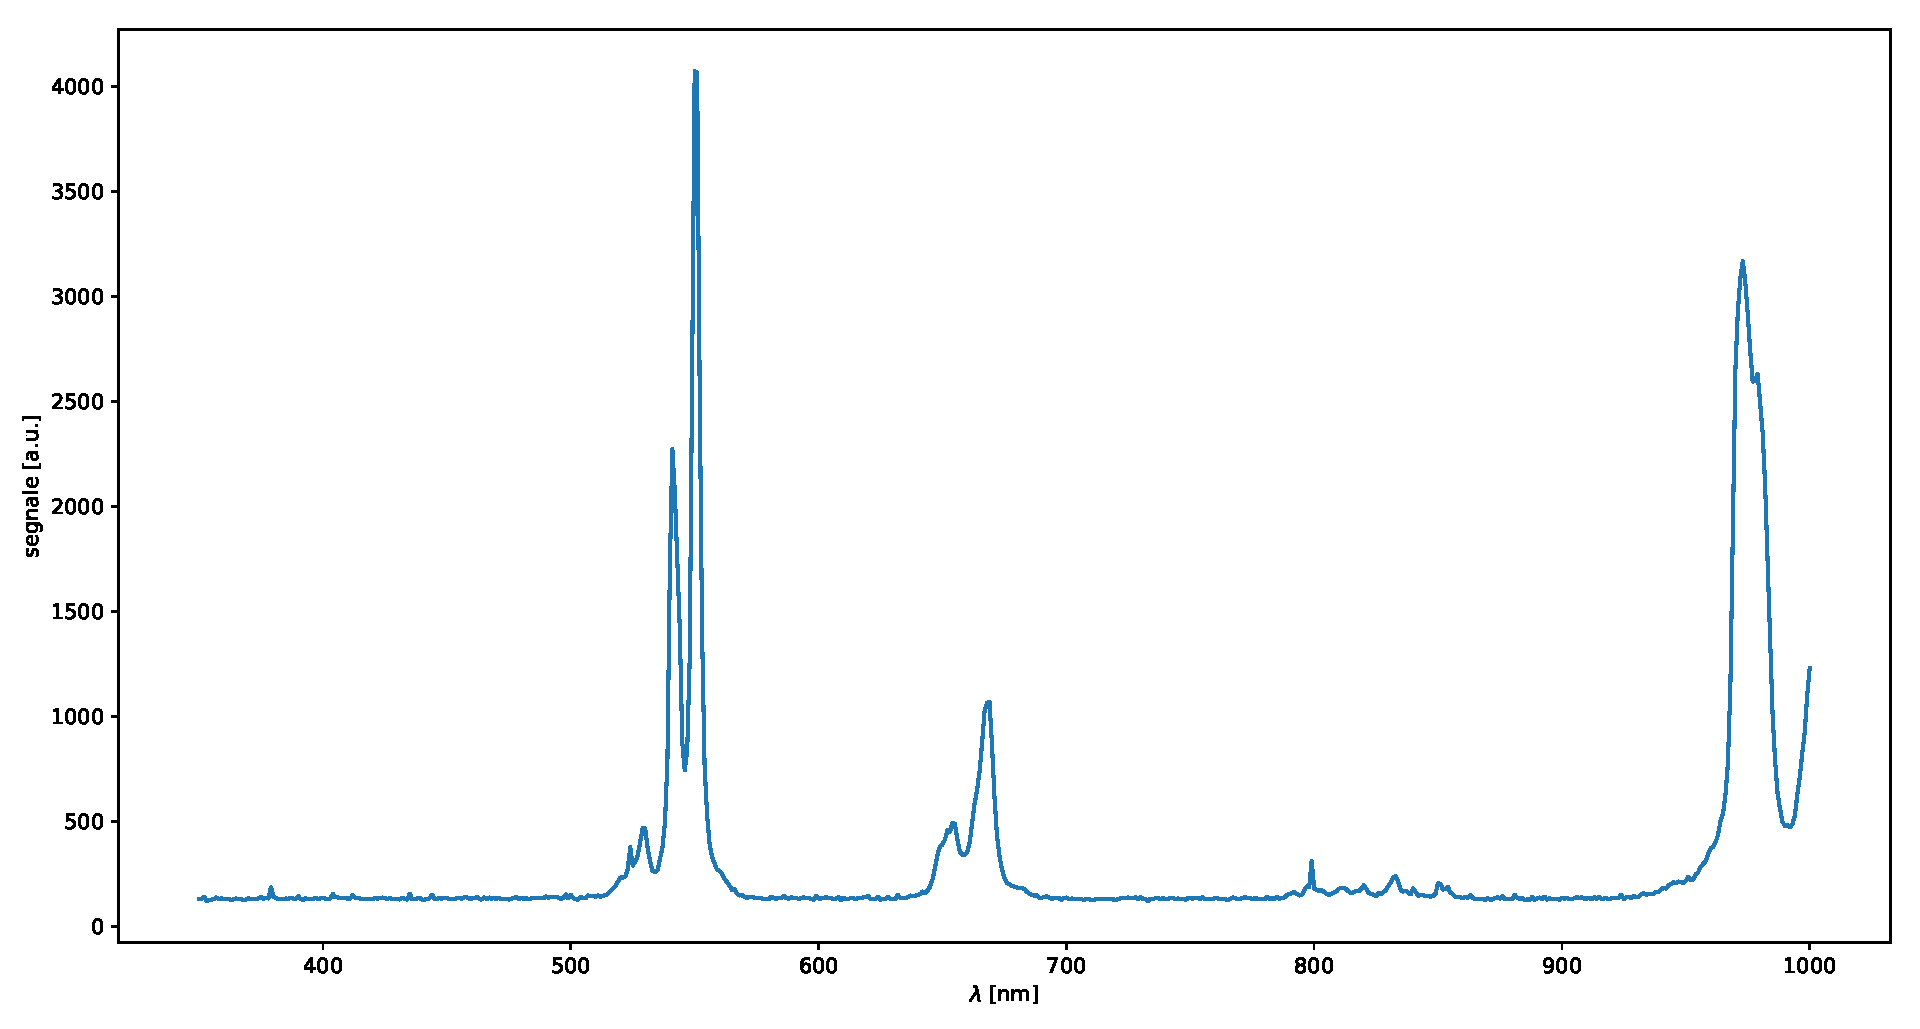
\includegraphics[width=\textwidth]{spettro}
\caption{Spettro di emissione del cristallo}
\label{fig:spettro}
\end{figure}

\begin{multicols}{2}

\section{Analisi dati}

\subsection{Bassa potenza}

2 fit: ax$^b$ e ax$^2$

\subsubsection{Analisi del cut}

grafico di b in funzione del cut

\subsection{Alta potenza}

1 fit lineare

\subsection{Spettro di emissione}

plot spettro
	
\end{multicols}

\newpage

\section*{Appendice}

\begin{table}[H]
\centering
\begin{tabular}{|cc|cc|cc|cc|cc|}
	$\theta$ [deg] & P [mW] & $\theta$ [deg] & P [mW] & $\theta$ [deg] & P [mW] & $\theta$ [deg]  & P [mW] & $\theta$ [deg]  & P [mW] \\
	\hline
240	&	462	&	166	&	941		&	92	&	4.72		&	20	&	21.77	&	308	&	116.1	\\
238	&	462	&	164	&	980		&	90	&	4.94		&	18	&	22.76	&	306	&	123.4	\\
236	&	463	&	162	&	1.021	&	88	&	5.16		&	16	&	23.70	&	304	&	131.1	\\
234	&	467	&	160	&	1.062	&	86	&	5.39		&	14	&	24.67	&	302	&	139.7	\\
232	&	470	&	158	&	1.111	&	84	&	5.63		&	12	&	25.87	&	300	&	148.2	\\
230	&	469	&	156	&	1.154	&	82	&	5.85		&	10	&	26.67	&	298	&	158.0	\\
228	&	470	&	154	&	1.216	&	80	&	6.13		&	8	&	27.87	&	296	&	171.1	\\
226	&	466	&	152	&	1.271	&	78	&	6.38		&	6	&	29.05	&	294	&	184.1	\\
224	&	467	&	150	&	1.320	&	76	&	6.62		&	4	&	30.3		&	292	&	196.0	\\
222	&	468	&	148	&	1.391	&	74	&	6.93		&	2	&	31.5		&	290	&	209.8	\\
220	&	469	&	146	&	1.440	&	72	&	7.23		&	0	&	32.8		&	288	&	223.8	\\
218	&	470	&	144	&	1.510	&	70	&	7.54		&	358	&	34.1		&	286	&	238.8	\\
216	&	469	&	142	&	1.586	&	68	&	7.86		&	356	&	35.6		&	284	&	257.8	\\
214	&	458	&	140	&	1.668	&	66	&	8.27		&	354	&	37.1		&	282	&	275.8	\\
212	&	413	&	138	&	1.744	&	64	&	8.66		&	352	&	38.8		&	280	&	296.0	\\
210	&	298	&	136	&	1.839	&	62	&	9.06		&	350	&	40.4		&	278	&	316	\\
208	&	145.0&	134	&	1.913	&	60	&	9.53		&	348	&	42.0		&	276	&	338	\\
206	&	45.2	&	132	&	1.988	&	58	&	9.93		&	346	&	43.9		&	274	&	361	\\
204	&	8.42	&	130	&	2.078	&	56	&	10.27	&	344	&	46.0		&	272	&	382	\\
202	&	1.763&	128	&	2.171	&	54	&	10.83	&	342	&	47.9		&	270	&	402	\\
200	&	897	&	126	&	2.270	&	52	&	11.36	&	340	&	50.1		&	268	&	433	\\
198	&	724	&	124	&	2.383	&	50	&	11.80	&	338	&	52.2		&	266	&	454	\\
196	&	624	&	122	&	2.497	&	48	&	12.12	&	336	&	54.3		&	264	&	464	\\
194	&	589	&	120	&	2.614	&	46	&	12.66	&	334	&	56.5		&	262	&	465	\\
192	&	586	&	118	&	2.733	&	44	&	13.18	&	332	&	58.9		&	260	&	466	\\
190	&	598	&	116	&	2.858	&	42	&	13.81	&	330	&	61.6		&	258	&	468	\\
188	&	614	&	114	&	3.01		&	40	&	14.44	&	328	&	64.4		&	256	&	467	\\
186	&	629	&	112	&	3.14		&	38	&	15.08	&	326	&	67.4		&	254	&	467	\\
184	&	650	&	110	&	3.29		&	36	&	15.67	&	324	&	70.0		&	252	&	467	\\
182	&	672	&	108	&	3.46		&	34	&	16.51	&	322	&	74.4		&	250	&	466	\\
180	&	696	&	106	&	3.60		&	32	&	17.22	&	320	&	79.0		&	248	&	469	\\
178	&	725	&	104	&	3.78		&	30	&	17.83	&	318	&	83.2		&	246	&	471	\\
176	&	755	&	102	&	3.95		&	28	&	18.60	&	316	&	87.2		&	244	&	471	\\
174	&	787	&	100	&	4.13		&	26	&	19.29	&	314	&	92.1		&	242	&	468	\\
172	&	821	&	98	&	4.34		&	24	&	20.05	&	312	&	97.5		&	240	&	464	\\
170	&	856	&	96	&	4.52		&	22	&	20.83	&	310	&	103.3	&	238	&	463	\\
168	&	898	&	94	&	4.72		&		&			&		&			&		&		\\	
\hline
\end{tabular}
\caption{Dati relativi alla taratura dell'attenuatore variabile. Gli errori di calibrazione sulle potenze sono del 3\%. L'errore sull'angolo � inferiore a 0.5 gradi centesimali, quindi � trascurabile.}
\label{tab:taratura}
\end{table}

\begin{table}[H]
\centering
\begin{tabular}{|ccc|ccc|ccc|ccc|}
$\theta$ [deg] & V$_{pp}$ [mV] & $\Delta$V$_{pp}$ & $\theta$ [deg] & V$_{pp}$ [mV] & $\Delta$V$_{pp}$ & $\theta$ [deg] & V$_{pp}$ [mV] & $\Delta$V$_{pp}$ & $\theta$ [deg]  & V$_{pp}$ [mV] & $\Delta$V$_{pp}$  \\
	\hline
240	&	500	&	20	&	322	&	66	&	2	&	12	&	14.8	&	0.8	&	60	&	2.3	&	0.2	\\
250	&	480	&	20	&	324	&	62	&	2	&	14	&	14.8	&	0.8	&	62	&	2.1	&	0.2	\\
254	&	480	&	20	&	326	&	60	&	2	&	16	&	14.0	&	0.8	&	64	&	1.9	&	0.2	\\
258	&	460	&	20	&	328	&	58	&	2	&	18	&	12.8	&	0.8	&	66	&	1.7	&	0.2	\\
262	&	460	&	20	&	330	&	50	&	2	&	20	&	12.4	&	0.8	&	68	&	1.8	&	0.2	\\
266	&	460	&	20	&	332	&	50	&	2	&	22	&	12.0	&	0.8	&	70	&	1.6	&	0.2	\\
270	&	420	&	20	&	334	&	48	&	2	&	24	&	11.2	&	0.8	&	72	&	1.5	&	0.2	\\
274	&	390	&	10	&	336	&	44	&	2	&	26	&	10.0	&	0.8	&	74	&	1.4	&	0.2	\\
278	&	350	&	10	&	338	&	42	&	2	&	28	&	9.2	&	0.8	&	76	&	1.3	&	0.2	\\
282	&	310	&	10	&	340	&	40	&	1	&	30	&	8.8	&	0.8	&	78	&	1.3	&	0.2	\\
286	&	270	&	10	&	342	&	38	&	1	&	32	&	8.0	&	0.8	&	80	&	1.1	&	0.2	\\
290	&	230	&	10	&	344	&	34	&	1	&	34	&	7.2	&	0.8	&	82	&	1.0	&	0.2	\\
294	&	200	&	10	&	346	&	32	&	1	&	36	&	6.4	&	0.4	&	84	&	0.9	&	0.2	\\
298	&	180	&	10	&	348	&	32	&	1	&	38	&	6.2	&	0.4	&	86	&	0.9	&	0.2	\\
300	&	170	&	10	&	350	&	31	&	1	&	40	&	5.8	&	0.4	&	88	&	0.8	&	0.2	\\
302	&	152	&	4	&	352	&	28	&	1	&	42	&	5.4	&	0.4	&	90	&	0.7	&	0.2	\\
304	&	128	&	4	&	354	&	25	&	1	&	44	&	4.8	&	0.4	&	92	&	0.6	&	0.2	\\
306	&	120	&	4	&	356	&	24	&	1	&	46	&	4.6	&	0.4	&	94	&	0.6	&	0.2	\\
308	&	116	&	4	&	358	&	22	&	1	&	48	&	4.4	&	0.4	&	96	&	0.5	&	0.2	\\
310	&	116	&	4	&	360	&	22	&	1	&	50	&	4.0	&	0.4	&	98	&	0.5	&	0.2	\\
312	&	104	&	4	&	2	&	20	&	1	&	52	&	3.6	&	0.2	&	100	&	0.5	&	0.2	\\
314	&	92	&	4	&	4	&	19	&	1	&	54	&	3.3	&	0.2	&	102	&	0.4	&	0.2	\\
316	&	80	&	2	&	6	&	19	&	1	&	56	&	2.9	&	0.2	&	104	&	0.4	&	0.2	\\
318	&	76	&	2	&	8	&	17	&	1	&	58	&	2.7	&	0.2	&	106	&	0.3	&	0.2	\\
320	&	72	&	2	&	10	&	14.8	&	0.8	&		&		&		&		&		&		\\
\hline
\end{tabular}
\caption{Dati relativi alla prima presa dati. Gli errori $\Delta$V$_{pp}$ sono relativi alle tacche dell'oscilloscopio. L'errore sull'angolo � inferiore a 0.5 gradi centesimali, quindi � trascurabile.}
\label{tab:primo}
\end{table}

\begin{table}[H]
\centering
\begin{tabular}{|ccc|ccc|ccc|ccc|}
$\theta$ [deg] & V$_{pp}$ [mV] & $\Delta$V$_{pp}$ & $\theta$ [deg] & V$_{pp}$ [mV] & $\Delta$V$_{pp}$ & $\theta$ [deg] & V$_{pp}$ [mV] & $\Delta$V$_{pp}$ & $\theta$ [deg]  & V$_{pp}$ [mV] & $\Delta$V$_{pp}$  \\
	\hline
270	&	2400	&	100	&	316	&	520	&	20	&	24	&	62	&	2	&	80	&	6.2	&	0.4	\\
280	&	1800	&	100	&	318	&	500	&	20	&	26	&	58	&	2	&	82	&	6.6	&	0.2	\\
284	&	1600	&	40	&	320	&	480	&	20	&	28	&	52	&	2	&	84	&	5.6	&	0.2	\\
288	&	1440	&	40	&	322	&	440	&	20	&	30	&	48	&	2	&	86	&	5.4	&	0.2	\\
292	&	1200	&	40	&	324	&	420	&	20	&	32	&	46	&	2	&	88	&	5.0	&	0.2	\\
296	&	1120	&	40	&	326	&	390	&	10	&	34	&	40	&	2	&	90	&	4.8	&	0.2	\\
300	&	960	&	40	&	328	&	370	&	10	&	36	&	38	&	2	&	92	&	4.6	&	0.2	\\
302	&	880	&	40	&	330	&	330	&	10	&	38	&	38	&	1	&	94	&	4.2	&	0.2	\\
240	&	2900	&	100	&	332	&	320	&	10	&	40	&	36	&	1	&	96	&	3.8	&	0.2	\\
250	&	2700	&	100	&	334	&	300	&	10	&	42	&	34	&	1	&	98	&	3.4	&	0.2	\\
256	&	2600	&	100	&	336	&	270	&	10	&	44	&	33	&	1	&	100	&	3.0	&	0.1	\\
260	&	2700	&	100	&	338	&	250	&	10	&	46	&	31	&	1	&	102	&	2.8	&	0.1	\\
264	&	2600	&	100	&	340	&	240	&	10	&	48	&	27	&	1	&	104	&	2.5	&	0.1	\\
268	&	2500	&	100	&	342	&	230	&	10	&	50	&	24	&	1	&	106	&	2.5	&	0.1	\\
272	&	2400	&	100	&	344	&	220	&	10	&	52	&	23	&	1	&	108	&	2.2	&	0.1	\\
276	&	2100	&	100	&	346	&	200	&	10	&	54	&	21	&	1	&	110	&	2.1	&	0.1	\\
282	&	1700	&	100	&	348	&	180	&	10	&	56	&	19	&	1	&	112	&	1.9	&	0.1	\\
286	&	1600	&	40	&	350	&	170	&	10	&	58	&	16	&	0.4	&	114	&	1.7	&	0.1	\\
290	&	1360	&	40	&	354	&	160	&	4	&	60	&	16	&	0.4	&	116	&	1.5	&	0.1	\\
294	&	1200	&	40	&	358	&	140	&	4	&	62	&	15.2	&	0.4	&	118	&	1.3	&	0.1	\\
298	&	1040	&	40	&	2	&	120	&	4	&	64	&	14	&	0.4	&	120	&	1.2	&	0.1	\\
302	&	920	&	40	&	6	&	116	&	4	&	66	&	13.2	&	0.4	&	122	&	1.1	&	0.1	\\
304	&	840	&	40	&	10	&	100	&	4	&	68	&	12.4	&	0.4	&	124	&	1.0	&	0.1	\\
306	&	760	&	40	&	12	&	92	&	4	&	70	&	10	&	0.4	&	126	&	0.9	&	0.1	\\
308	&	720	&	40	&	16	&	80	&	4	&	72	&	8.8	&	0.4	&	128	&	0.8	&	0.1	\\
310	&	680	&	40	&	18	&	74	&	2	&	74	&	8.2	&	0.4	&	130	&	0.7	&	0.1	\\
312	&	640	&	40	&	20	&	68	&	2	&	76	&	8.0	&	0.4	&	132	&	0.7	&	0.1	\\
314	&	600	&	40	&	22	&	64	&	2	&	78	&	7.8	&	0.4	&	136	&	0.6	&	0.1	\\\hline
\end{tabular}
\caption{Dati relativi alla seconda presa dati. Gli errori $\Delta$V$_{pp}$ sono relativi alle tacche dell'oscilloscopio. L'errore sull'angolo � inferiore a 0.5 gradi centesimali, quindi � trascurabile.}
\label{tab:secondo}
\end{table}

\end{document}